\documentclass[conference]{IEEEtran}
\IEEEoverridecommandlockouts
\usepackage{cite}
\usepackage{amsmath,amssymb,amsfonts}
\usepackage{algorithmic}
\usepackage{graphicx}
\usepackage{textcomp}
\usepackage{xcolor}
\usepackage{tikz}
\usepackage{pgfgantt}
\usetikzlibrary{shapes.geometric, arrows, positioning}

% Define colors
\definecolor{lightblue}{RGB}{173,216,230}
\definecolor{lightgreen}{RGB}{144,238,144}
\definecolor{lightyellow}{RGB}{255,255,224}

\begin{document}

\title{Cross-Platform Performance Analysis of Modern Neural Networks: A JAX-Centric Hardware-Software Co-Design Study}

\author{\IEEEauthorblockN{Sanchez Shiromizu L.T, Shashwat S, Prathyush B, Sai M}
\IEEEauthorblockA{\{lsanc68, ssinha30, pball5, sbadr4\}@uic.edu}
\IEEEauthorblockA{\textit{ECE 594 HW-SW Co-Design for ML Systems} \\
\textit{University of Illinois at Chicago}\\
Chicago, IL}
}

\maketitle

\section{Introduction and Motivation}

The deployment of machine learning models requires careful selection of both hardware platforms (CPUs, GPUs, TPUs)
 and software frameworks (JAX, PyTorch, TensorFlow), yet guidance for these decisions remains surprisingly scarce 
 \cite{menghani2023efficient, bianco2018benchmark}. While scattered benchmarks exist online, they frequently suffer
  from outdated methodologies, inconsistent testing procedures, or narrow platform coverage. This fragmentation 
  makes it difficult to understand how architectural choices such as traditional CNNs versus modern Transformers
   in different frameworks impact performance across diverse hardware configurations.

From a hardware and software co-design perspective, this knowledge gap presents significant challenges. Understanding
 the relationship between architectural decisions and accelerator characteristics is critical during design and 
 development of machine learning systems \cite{guo2024survey, krishna2025hwswcodesign}, particularly as specialized
  hardware like TPUs becomes increasingly prevalent in production environments \cite{jouppi2023tpuv4, omdia2024tpu}.
   The consequences of suboptimal choices are substantial: the use of incorrect framework and hardware pairings can
    lead to 2-10$\times$ waste in computational resources and development time 
    \cite{strubell2019energy, patterson2021carbon, mlsysbook2024}. Without identifying true performance 
    bottlenecks, engineering teams risk investing months optimizing non-critical system components.

\section{Related Work and Gaps}

Existing benchmarking provide valuable insights but show significant limitations. MLPerf Benchmarks 
\cite{mlperf2020} establish standards for performance measurements, yet predominantly emphasize training 
results over inference and exclude JAX entirely. DAWNBench \cite{coleman2017} offered comprehensive analysis 
at its release in 2017 but now lacks coverage of contemporary architectures such as Vision Transformers and modern
 accelerators including TPUs. Benchmarks from PyTorch and TensorFlow documentation offer useful 
 reference points for implementation and reference performance levels but typically present optimistic values
  without independent verification.

 A fundamental limitation across existing benchmarks is their focus on \textit{what} performs better rather than 
 \textit{why} performance differences occur \cite{wang2019benchmarking, zhao2017layerwise}. Questions about memory 
  bandwidth versus compute bottlenecks remain unexplored, yet this understanding is essential for 
   hardware and software co-design \cite{cho2020accelerating, bianco2018benchmark}. Additionally, most 
  benchmarks optimize for single metrics (typically throughput) while neglecting other deployment-critical factors
   including memory footprint, energy efficiency, and compilation overhead 
   \cite{canziani2019deployment, benmeziane2021comprehensive, ignatov2018aibenchmark}.

\begin{figure}[t]
\centering
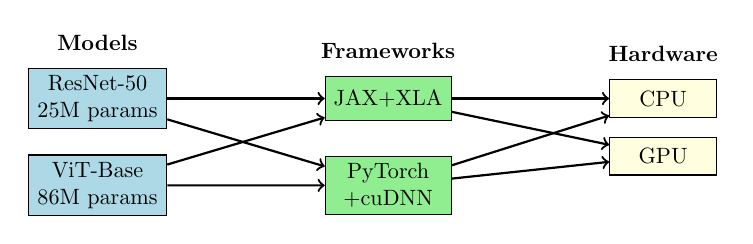
\begin{tikzpicture}[node distance=1.5cm, scale=0.8, transform shape]
    % Models
    \node[rectangle, draw, fill=lightblue, minimum width=2.2cm, minimum height=0.9cm, align=center] (resnet) {ResNet-50\\25M params};
    \node[rectangle, draw, fill=lightblue, minimum width=2.2cm, minimum height=0.9cm, below=0.4cm of resnet, align=center] (vit) {ViT-Base\\86M params};
    
    % Frameworks
    \node[rectangle, draw, fill=lightgreen, minimum width=2cm, minimum height=0.7cm, right=2.5cm of resnet, align=center] (jax) {JAX+XLA};
    \node[rectangle, draw, fill=lightgreen, minimum width=2cm, minimum height=0.7cm, right=2.5cm of vit, align=center] (pytorch) {PyTorch\\+cuDNN};
    
    % Hardware
    \node[rectangle, draw, fill=lightyellow, minimum width=1.7cm, minimum height=0.6cm, right=2.5cm of jax] (cpu) {CPU};
    \node[rectangle, draw, fill=lightyellow, minimum width=1.7cm, minimum height=0.6cm, below=0.3cm of cpu] (gpu) {GPU};
    
    % Arrows
    \draw[->, thick] (resnet) -- (jax);
    \draw[->, thick] (resnet) -- (pytorch);
    \draw[->, thick] (vit) -- (jax);
    \draw[->, thick] (vit) -- (pytorch);
    
    \draw[->, thick] (jax) -- (cpu);
    \draw[->, thick] (jax) -- (gpu);
    \draw[->, thick] (pytorch) -- (cpu);
    \draw[->, thick] (pytorch) -- (gpu);
    
    % Labels
    \node[above=0.15cm of resnet] {\textbf{Models}};
    \node[above=0.15cm of jax] {\textbf{Frameworks}};
    \node[above=0.15cm of cpu] {\textbf{Hardware}};
\end{tikzpicture}
\caption{Focused system architecture: 2 models $\times$ 2 frameworks $\times$ 2 platforms = 8 configurations to benchmark and analyze. TPU evaluation as optional extension if time permits.}
\label{fig:architecture}
\end{figure}

\section{Proposed Approach}

We propose a focused study that addresses the critical gaps through systematic analysis of two representative
 neural network architectures across two frameworks and two hardware platforms, as illustrated in Figure 
 \ref{fig:architecture}. This reduced scope enables deeper analysis of each configuration while maintaining 
 project feasibility within the 8-week timeline.

\textbf{ResNet-50} will establish our baseline, representing conventional convolutional architectures with 25M parameters
and approximately 4 GFLOPs of computation. Its compute-bound characteristics on modern hardware will provide a reference
for understanding standard CNN performance patterns across frameworks and platforms.

\textbf{Vision Transformer Base} will represent contemporary attention based architectures with 86M parameters and 
quadratic memory usage in self-attention mechanisms. This architecture stresses memory systems differently 
than CNNs, providing critical insights into how JAX handles attention operations compared to PyTorch's optimized 
implementations.

Our implementation approach will begin with native JAX implementations, providing complete control over architectural 
details. We will validate against reference implementations from torchvision, which is widely used in the community 
with well-established benchmarks. Benchmarking will span CPU baselines and NVIDIA GPUs (H100NVL) as primary platforms, 
with Google TPUs (v3 or v4) as an optional extension if time and resources permit. For each configuration, we will 
measure:

\begin{itemize}
    \item \textbf{Latency}: Single sample inference time (critical for real-time applications)
    \item \textbf{Throughput}: Samples per second at batch sizes [1, 8, 32, 128]
    \item \textbf{Memory}: Peak memory usage during inference
    \item \textbf{Compilation time}: How long XLA/JIT takes (affects development iteration speed)
    \item \textbf{Energy}: Power consumption where measurable (nvidia-smi for GPUs)
\end{itemize}

Our methodology will emphasize understanding of performance differences through testing. We will employ
tools including XLA profiler and TensorBoard to identify whether configurations are compute bound, memory 
bandwidth limited, or constrained by host to device transfers. This focused analysis will provide actionable 
insights for practitioners choosing between JAX and PyTorch for different deployment scenarios.

\section{Advantages Over Existing Work}

Our work advances beyond existing benchmarks by focusing on a critical question: \textbf{How does JAX compare 
to PyTorch across different hardware platforms?} This focused approach enables several key contributions.

First, we incorporate modern architectures including Vision Transformers, which have gained widespread adoption 
in the community \cite{papa2024efficient, han2023survey} despite limited presence in established benchmarks 
\cite{mlperf2020, coleman2017}. Second, we will ensure consistent model implementations 
and optimization levels across both frameworks (Using JAX hability to be highly custimizable), eliminating variables that could potentially confound the results.

Third, we provide the first systematic evaluation of JAX performance against PyTorch the most widely adopted 
framework across diverse hardware platforms. While JAX adoption has accelerated in research contexts, notably 
in DeepMind's AlphaFold \cite{jumper2021alphafold, deepmind2021jax}, practical performance guidance remains 
limited. Our work directly addresses this gap.

Fourth, our analysis extends beyond raw performance metrics to investigate architectural interactions with hardware.
We examine how attention mechanisms in Vision Transformers behave differently across frameworks and platforms, 
and whether JAX's XLA compilation provides advantages over PyTorch's eager execution and JIT capabilities.

Finally, we ensure complete reproducibility through open source code release, comprehensive documentation,
and transparent methodology, enabling independent verification and extension to additional architectures or
platforms.


\section{Implementation Plan}

We structure the project into five phases spanning 8 weeks from October 20 to December 10, 2025, as shown in 
Figure \ref{fig:timeline}. The focused scope allows deeper investigation of each configuration while maintaining 
an achievable timeline.

\textbf{Week 1 (Oct 20-26, Setup)}: Environment configuration for JAX and PyTorch on available GPU 
infrastructure. Initial model implementations starting with ResNet-50. 
We utilize ImageNet pre-trained weights as starting points for validation. Optional: Submit TPU access 
application for potential extension work.

\textbf{Weeks 2-3 (Oct 27-Nov 9, Implementation \& Infrastructure)}: Complete native JAX implementations of both 
architectures with numerical validation against PyTorch reference implementations (tolerance: 1e-5 for FP32). 
Simultaneously develop benchmarking infrastructure incorporating warmup periods (10 iterations), 
measurement iterations (minimum 50), and automated logging. Begin baseline measurements for initial configurations.

\textbf{Weeks 4-5 (Nov 10-23, Data Collection)}: Comprehensive benchmarking period with minimum 50 iterations per 
configuration to ensure statistical significance. Evaluate across varying batch sizes and precision levels (FP32, 
FP16/BF16). Apply framework specific optimizations and conduct profiling using nvprof (GPU) and perf (CPU). 
Complete all 8 primary configurations (2 models $\times$ 2 frameworks $\times$ 2 platforms). If TPU access 
granted, conduct preliminary TPU benchmarks.

\textbf{Weeks 6-7 (Nov 24-Dec 7, Analysis \& Documentation)}: Deep analysis of results focusing on the core question: 
how and why JAX and PyTorch perform differently across platforms. Construct performance comparison matrices, 
generate visualizations (heatmaps, roofline plots, scaling curves), and investigate architectural hypotheses. 
Simultaneously prepare report with detailed methodology and results sections.

\textbf{Week 8 (Dec 8-12, Finalization)}: Final presentation preparation focusing on key insights, codebase 
refinement, integration of feedback, and repository documentation. Presentation delivery by December 10, 2025.

\begin{figure}[b]
\centering
\begin{ganttchart}[
    hgrid,
    vgrid,
    x unit=0.68cm,
    y unit title=0.5cm,
    y unit chart=0.4cm,
    title height=1,
    bar/.append style={fill=lightblue},
    bar height=0.6,
    group height=0.4
]{1}{8}
\gantttitle{Project Timeline: Oct 20 - Dec 10, 2025}{8} \\
\gantttitlelist{1,...,8}{1} \\
\ganttbar{Setup}{1}{1} \\
\ganttbar{Impl. \& Infra.}{2}{3} \\
\ganttbar{Data Collection}{4}{5} \\
\ganttbar{Analysis \& Docs}{6}{7} \\
\ganttbar{Finalization}{8}{8}
\end{ganttchart}
\caption{Accelerated 8-week timeline from October 20 to December 10, 2025, with overlapping phases for efficiency.}
\label{fig:timeline}
\end{figure}

\section{Resources and Risk Mitigation}

Required resources include GPU access (university cluster 4xH100NVL), ImageNet-100 dataset (approximately 50GB, 
providing 100-class subset with sufficient complexity while remaining manageable), and approximately 120 GPU-hours 
distributed across implementation (30h), benchmarking (50h), optimization experiments (25h), and analysis (15h).

The focused scope significantly reduces risk. With only 8 primary configurations instead of 27, we can achieve 
statistical significance (100+ iterations per configuration) while maintaining schedule buffer. Dataset choice 
of ImageNet-100 provides a middle ground: substantially more representative than Tiny-ImageNet (500MB) while 
avoiding the 150GB storage and processing overhead of full ImageNet.

TPU access remains optional. If granted within Week 2-3, we add 4 configurations as extension work. If not 
granted, the core CPU/GPU comparison across JAX and PyTorch remains complete and scientifically valid.

Team division of labor: Member 1 focuses on JAX implementations, Member 2 on PyTorch baselines, Member 3 on 
benchmarking infrastructure, and Member 4 on analysis and visualization. This parallel approach maximizes 
efficiency while maintaining quality control through peer review.

Contingency plans: If hardware access issues arise, cloud GPU credits (Google Colab Pro, AWS, or Azure) provide 
fallback. If ImageNet-100 proves problematic, CIFAR-100 serves as final fallback while maintaining the comparative 
framework analysis.

\begin{thebibliography}{00}
    \bibitem{mlperf2020} P. Mattson et al., ``MLPerf Training Benchmark,'' in \textit{Proc. Machine Learning and Systems (MLSys)}, vol. 2, pp. 336-349, 2020.
    
    \bibitem{coleman2017} C. Coleman et al., ``DAWNBench: An End-to-End Deep Learning Benchmark and Competition,'' in \textit{NIPS ML Systems Workshop}, 2017.
    
    \bibitem{menghani2023efficient} G. Menghani, ``Efficient Deep Learning: A Survey on Making Deep Learning Models Smaller, Faster, and Better,'' \textit{ACM Computing Surveys}, vol. 55, no. 12, pp. 1-37, 2023.
    
    \bibitem{bianco2018benchmark} S. Bianco, R. Cadene, L. Celona, and P. Napoletano, ``Benchmark Analysis of Representative Deep Neural Network Architectures,'' \textit{IEEE Access}, vol. 6, pp. 64270-64277, 2018.
    
    \bibitem{guo2024survey} C. Guo et al., ``A Survey: Collaborative Hardware and Software Design in the Era of Large Language Models,'' \textit{arXiv preprint arXiv:2410.07265}, 2024.
    
    \bibitem{krishna2025hwswcodesign} T. Krishna, ``Hardware Software Co-Design for Machine Learning Systems,'' Course Materials, Georgia Institute of Technology, 2025.
    
    \bibitem{jouppi2023tpuv4} N. P. Jouppi et al., ``TPU v4: An Optically Reconfigurable Supercomputer for Machine Learning,'' in \textit{Proc. 50th ISCA}, 2023.
    
    \bibitem{omdia2024tpu} A. Harrowell, ``Demand for Google's TPU Chips Accelerates,'' Omdia Research Report, December 2024.
    
    \bibitem{strubell2019energy} E. Strubell, A. Ganesh, and A. McCallum, ``Energy and Policy Considerations for Deep Learning in NLP,'' in \textit{Proc. 57th ACL}, pp. 3645-3650, 2019.
    
    \bibitem{patterson2021carbon} D. Patterson et al., ``Carbon Emissions and Large Neural Network Training,'' \textit{arXiv:2104.10350}, 2021.
    
    \bibitem{mlsysbook2024} ``Sustainable AI,'' in \textit{Machine Learning Systems: Design and Implementation}, 2024.
    
    \bibitem{bradbury2018jax} J. Bradbury et al., ``JAX: Composable Transformations of Python+NumPy Programs,'' 2018.
    
    \bibitem{vaswani2017attention} A. Vaswani et al., ``Attention is All You Need,'' in \textit{NeurIPS}, vol. 30, 2017.
    
    \bibitem{wang2019benchmarking} Y. Wang et al., ``Benchmarking TPU, GPU, and CPU Platforms for Deep Learning,'' \textit{arXiv:1907.10701}, 2019.
    
    \bibitem{zhao2017layerwise} H. Zhao, C. Cartledge, and A. Jog, ``Layer-wise Performance Bottleneck Analysis,'' in \textit{Proc. AIM}, 2017.
    
    \bibitem{cho2020accelerating} B. Y. Cho, J. Jung, and M. Erez, ``Accelerating Bandwidth-Bound Deep Learning Inference,'' in \textit{Proc. SC}, pp. 1-14, 2020.
    
    \bibitem{canziani2019deployment} A. Canziani, A. Paszke, and E. Culurciello, ``An Analysis of Deep Neural Network Models for Practical Applications,'' \textit{arXiv:1605.07678}, 2019.
    
    \bibitem{benmeziane2021comprehensive} H. Benmeziane et al., ``A Comprehensive Survey on Hardware-Aware Neural Architecture Search,'' \textit{arXiv:2101.09336}, 2021.
    
    \bibitem{ignatov2018aibenchmark} A. Ignatov et al., ``AI Benchmark: Running Deep Neural Networks on Android Smartphones,'' in \textit{Proc. ECCV Workshops}, 2018.
    
    \bibitem{papa2024efficient} L. Papa et al., ``A Survey on Efficient Vision Transformers,'' \textit{IEEE TPAMI}, vol. 46, no. 12, pp. 7682-7700, 2024.
    
    \bibitem{han2023survey} K. Han et al., ``A Survey on Vision Transformer,'' \textit{IEEE TPAMI}, vol. 45, no. 1, pp. 87-110, 2023.
    
    \bibitem{jumper2021alphafold} J. Jumper et al., ``Highly Accurate Protein Structure Prediction with AlphaFold,'' \textit{Nature}, vol. 596, pp. 583-589, 2021.
    
    \bibitem{deepmind2021jax} ``Using JAX to Accelerate Our Research,'' DeepMind Blog, 2020.
    
    \bibitem{qin2018diagonalwise} H. Qin et al., ``Forward and Backward Information Retention for Accurate Binary Neural Networks,'' in \textit{Proc. CVPR}, pp. 2250-2258, 2018.
    
    \bibitem{discuss2019depthwise} ``No Speedup with Depthwise Convolutions,'' PyTorch Forums, 2019.
\end{thebibliography}

\end{document}